%!TEX root = Problems2_main.tex

\makeatletter
\renewcommand{\@maketitle}{
\newpage
 \null
 \vskip 2em%
 \begin{center}%
  {\Large \@title \par}%
 \end{center}%
 \par} \makeatother

\begin{center}
\Huge University Physics Problems 2\\[1em]
\large March 2013
\end{center}

\section{Reflecting}
Two periscopes are constructed as shown below. In each case, the periscope is used to observe a person with the word BEN written on their t-shirt. In each case, the light is reflected from mirror 1 to mirror 2 and then to the observer. For each design, what is the orientation of the word as viewed by the observer?
\begin{figure}[ht]
  \centering
  %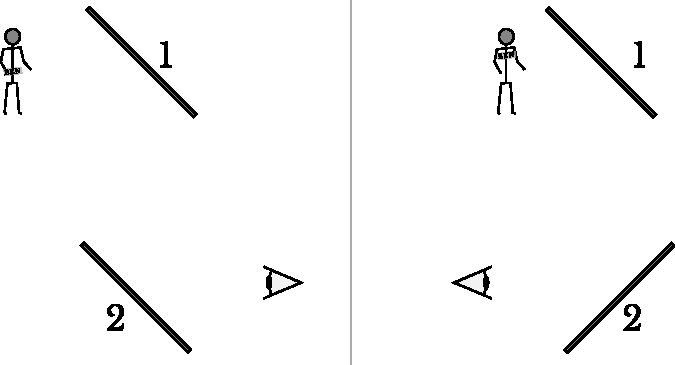
\includegraphics[width=0.3\textwidth]{periscopes.pdf}
\end{figure}

\section{Recombining}
A narrow beam of white light passes through a glass prism. The light is dispersed into its constituent colours. Can these rays be recombined into white light by passing them through a second prism?

\section{Throwing}
\begin{wrapfigure}{r}{0.4\textwidth}
  \vspace{-20pt}
  \begin{center}
  	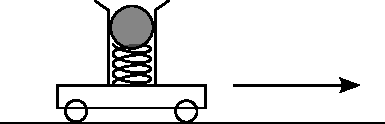
\includegraphics[width=0.38\textwidth]{trolley1.pdf}
  \end{center}
  \vspace{-20pt}
\end{wrapfigure}
A trolley rolls without friction along a track. When the trolley passes over some point in the track, the ball is released and is ejected upwards. Does it fall 
\begin{enumerate}[label=\alph*)]
	\item infront of the tube,
	\item behind the trube,
	\item back into the tube?
\end{enumerate}

\section{}
\begin{wrapfigure}{r}{0.4\textwidth}
  \vspace{-20pt}
  \begin{center}
  	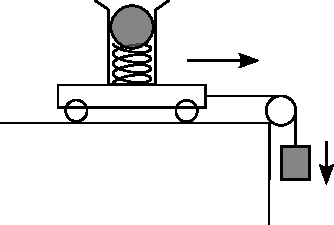
\includegraphics[width=0.38\textwidth]{trolley2.pdf}
  \end{center}
  \vspace{-20pt}
\end{wrapfigure}
The trolley is now connected via a light string and a pulley whell to a weight and the experiement repeated. Does the ball fall
\begin{enumerate}[label=\alph*)]
	\item infront of the tube,
	\item behind the trube,
	\item back into the tube?
\end{enumerate}

\section{}
\begin{wrapfigure}{r}{0.4\textwidth}
  \vspace{-20pt}
  \begin{center}
  	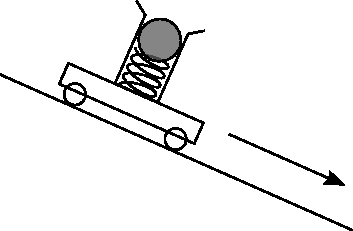
\includegraphics[width=0.38\textwidth]{trolley3.pdf}
  \end{center}
  \vspace{-20pt}
\end{wrapfigure}
Finally, the trolley is allowed to accelerate freely down an inclined plane. Does the ball fall
\begin{enumerate}[label=\alph*)]
	\item infront of the tube,
	\item behind the trube,
	\item back into the tube?
\end{enumerate}
